\documentclass{article}\usepackage[]{graphicx}\usepackage[]{color}
%% maxwidth is the original width if it is less than linewidth
%% otherwise use linewidth (to make sure the graphics do not exceed the margin)
\makeatletter
\def\maxwidth{ %
  \ifdim\Gin@nat@width>\linewidth
    \linewidth
  \else
    \Gin@nat@width
  \fi
}
\makeatother

\definecolor{fgcolor}{rgb}{0.345, 0.345, 0.345}
\newcommand{\hlnum}[1]{\textcolor[rgb]{0.686,0.059,0.569}{#1}}%
\newcommand{\hlstr}[1]{\textcolor[rgb]{0.192,0.494,0.8}{#1}}%
\newcommand{\hlcom}[1]{\textcolor[rgb]{0.678,0.584,0.686}{\textit{#1}}}%
\newcommand{\hlopt}[1]{\textcolor[rgb]{0,0,0}{#1}}%
\newcommand{\hlstd}[1]{\textcolor[rgb]{0.345,0.345,0.345}{#1}}%
\newcommand{\hlkwa}[1]{\textcolor[rgb]{0.161,0.373,0.58}{\textbf{#1}}}%
\newcommand{\hlkwb}[1]{\textcolor[rgb]{0.69,0.353,0.396}{#1}}%
\newcommand{\hlkwc}[1]{\textcolor[rgb]{0.333,0.667,0.333}{#1}}%
\newcommand{\hlkwd}[1]{\textcolor[rgb]{0.737,0.353,0.396}{\textbf{#1}}}%
\let\hlipl\hlkwb

\usepackage{framed}
\makeatletter
\newenvironment{kframe}{%
 \def\at@end@of@kframe{}%
 \ifinner\ifhmode%
  \def\at@end@of@kframe{\end{minipage}}%
  \begin{minipage}{\columnwidth}%
 \fi\fi%
 \def\FrameCommand##1{\hskip\@totalleftmargin \hskip-\fboxsep
 \colorbox{shadecolor}{##1}\hskip-\fboxsep
     % There is no \\@totalrightmargin, so:
     \hskip-\linewidth \hskip-\@totalleftmargin \hskip\columnwidth}%
 \MakeFramed {\advance\hsize-\width
   \@totalleftmargin\z@ \linewidth\hsize
   \@setminipage}}%
 {\par\unskip\endMakeFramed%
 \at@end@of@kframe}
\makeatother

\definecolor{shadecolor}{rgb}{.97, .97, .97}
\definecolor{messagecolor}{rgb}{0, 0, 0}
\definecolor{warningcolor}{rgb}{1, 0, 1}
\definecolor{errorcolor}{rgb}{1, 0, 0}
\newenvironment{knitrout}{}{} % an empty environment to be redefined in TeX

\usepackage{alltt}
%\usepackage{sober}
\usepackage{hyperref}
\usepackage[english]{babel}
\usepackage{amsmath}
\usepackage{natbib}
\newcommand{\code}[1]{{\tt #1}}
%\newcommand{\fixme}[1]{{\textbf #1}}
\newcommand{\multinom}{{\cal M}}
\date{\today}
\newcommand{\fixme}[1]{\textbf{FIXME: #1}}
\title{Mosquito combinatorics (occupancy spectrum)}
\author{Ben Bolker, with help from Leonid Bogachev,
  Ethan Bolker, and Ira Gessel}
\IfFileExists{upquote.sty}{\usepackage{upquote}}{}
\begin{document}
\bibliographystyle{chicago}

\maketitle

\textbf{Version: Sat Nov 18 15:16:42 2017}



\section{Preliminaries}

\begin{knitrout}
\definecolor{shadecolor}{rgb}{0.969, 0.969, 0.969}\color{fgcolor}\begin{kframe}
\begin{alltt}
\hlkwd{library}\hlstd{(rbenchmark)}
\hlkwd{library}\hlstd{(plyr)} \hlcom{## for laply}
\end{alltt}


{\ttfamily\noindent\color{warningcolor}{\#\# Warning: package 'plyr' was built under R version 3.2.5}}\begin{alltt}
\hlkwd{library}\hlstd{(plotrix)}
\end{alltt}


{\ttfamily\noindent\color{warningcolor}{\#\# Warning: package 'plotrix' was built under R version 3.2.5}}\begin{alltt}
\hlkwd{library}\hlstd{(reshape2)}
\end{alltt}


{\ttfamily\noindent\color{warningcolor}{\#\# Warning: package 'reshape2' was built under R version 3.2.5}}\begin{alltt}
\hlkwd{library}\hlstd{(abind)}
\end{alltt}


{\ttfamily\noindent\color{warningcolor}{\#\# Warning: package 'abind' was built under R version 3.2.5}}\begin{alltt}
\hlkwd{library}\hlstd{(ggplot2);} \hlkwd{theme_set}\hlstd{(}\hlkwd{theme_bw}\hlstd{())}
\end{alltt}


{\ttfamily\noindent\color{warningcolor}{\#\# Warning: package 'ggplot2' was built under R version 3.2.5}}\begin{alltt}
  \hlcom{## tweak to squash panels togethe}
\hlstd{zmargin} \hlkwb{<-} \hlkwd{theme}\hlstd{(}\hlkwc{panel.spacing}\hlstd{=grid}\hlopt{::}\hlkwd{unit}\hlstd{(}\hlnum{0}\hlstd{,}\hlstr{"lines"}\hlstd{))}
\hlkwd{library}\hlstd{(grid)}
\hlkwd{library}\hlstd{(numDeriv)}
\end{alltt}


{\ttfamily\noindent\color{warningcolor}{\#\# Warning: package 'numDeriv' was built under R version 3.2.5}}\end{kframe}
\end{knitrout}
\section{Introduction}
Suppose $B$=number of birds (bins); $M$=number of mosquitoes (balls).
$V$ is the (unordered) occupancy of a particular configuration
(e.g. $\{3,1,1,0\}$ means one bird sampled three times, two
birds sampled once, one bird not sampled);
$S=\{s_i\}$=occupancy spectrum (number of birds sampled $i$ times,
e.g. $S=\{1,2,0,1\}$ for the previous example).
The number of birds sampled at least once is 
$K=B-s_0=B-\sum_{i=1} s_i$.

We have $|V| = \sum s_i=B$;  $\sum v_i = \sum i s_i = M$.

Define the multinomial coefficient $\multinom(S) \equiv 
\binom{(\sum s_i)!}{\prod s_i!}$ \fixme{check? frac, not binom?}

Then the likelihood of observing an occupancy spectrum $S$ is
\begin{equation}
P(S|B,M) =  \frac{1}{B^M} \multinom(S) \multinom(V)
\end{equation}
where $\multinom(V)$ can also be written as
$M!/\prod_i (i!)^{s_i}$.

These are standard \emph{Maxwell-Boltzmann} statistics (as opposed
to some of the previous formulae, which were essentially Einstein-Bose
type, incorrectly [for this problem] treating some configurations
as equivalently).

\section{Code}
\subsection{Analytical formula}
The following functions implement this idea
(allowing for the possibility of returning
the log-probability, and allowing the possibility
of specifying the occupancy spectrum with the $s_0$
element excluded --- and filling it in using $s_0=B-K$).
\begin{knitrout}
\definecolor{shadecolor}{rgb}{0.969, 0.969, 0.969}\color{fgcolor}\begin{kframe}
\begin{alltt}
\hlcom{## multinomial coefficient}
\hlstd{mchoose} \hlkwb{<-} \hlkwa{function}\hlstd{(}\hlkwc{n}\hlstd{,}\hlkwc{log}\hlstd{=}\hlnum{FALSE}\hlstd{) \{}
    \hlstd{m} \hlkwb{<-} \hlkwd{lfactorial}\hlstd{(}\hlkwd{sum}\hlstd{(n))}\hlopt{-}\hlkwd{sum}\hlstd{(}\hlkwd{lfactorial}\hlstd{(n))}
    \hlkwa{if} \hlstd{(log) m} \hlkwa{else} \hlkwd{exp}\hlstd{(m)}
\hlstd{\}}
\hlstd{occprob} \hlkwb{<-} \hlkwa{function}\hlstd{(}\hlkwc{n}\hlstd{,}\hlkwc{B}\hlstd{,}\hlkwc{M}\hlstd{,}\hlkwc{log}\hlstd{=}\hlnum{FALSE}\hlstd{,}\hlkwc{add.zero}\hlstd{=}\hlnum{TRUE}\hlstd{) \{}
    \hlkwa{if} \hlstd{(add.zero) nx} \hlkwb{<-} \hlkwd{c}\hlstd{(B}\hlopt{-}\hlkwd{sum}\hlstd{(n),n)} \hlkwa{else} \hlstd{\{}
        \hlstd{nx} \hlkwb{<-} \hlstd{n; n} \hlkwb{<-} \hlstd{n[}\hlopt{-}\hlnum{1}\hlstd{]}
    \hlstd{\}}
    \hlstd{r} \hlkwb{<-} \hlopt{-}\hlstd{M}\hlopt{*}\hlkwd{log}\hlstd{(B)}\hlopt{+}\hlkwd{mchoose}\hlstd{(nx,}\hlkwc{log}\hlstd{=}\hlnum{TRUE}\hlstd{)}\hlopt{+}
        \hlkwd{lfactorial}\hlstd{(M)}\hlopt{-}\hlkwd{sum}\hlstd{(n}\hlopt{*}\hlkwd{lfactorial}\hlstd{(}\hlkwd{seq_along}\hlstd{(n)))}
    \hlkwa{if} \hlstd{(log) r} \hlkwa{else} \hlkwd{exp}\hlstd{(r)}
\hlstd{\}}
\end{alltt}
\end{kframe}
\end{knitrout}

\subsection{Simulation}
I simulated one realization of the process by
sampling birds with replacement and counting the number of occurrences
of each bird.

This can be done using \code{sample()} and then tabulating the results:
\begin{knitrout}
\definecolor{shadecolor}{rgb}{0.969, 0.969, 0.969}\color{fgcolor}\begin{kframe}
\begin{alltt}
\hlstd{vfun0} \hlkwb{<-} \hlkwa{function}\hlstd{(}\hlkwc{B}\hlstd{,}\hlkwc{M}\hlstd{)} \hlkwd{table}\hlstd{(}\hlkwd{factor}\hlstd{(}\hlkwd{sample}\hlstd{(}\hlnum{1}\hlopt{:}\hlstd{B,}\hlkwc{size}\hlstd{=M,}\hlkwc{replace}\hlstd{=}\hlnum{TRUE}\hlstd{),}\hlkwc{levels}\hlstd{=}\hlnum{1}\hlopt{:}\hlstd{B))}
\hlcom{#Result is Vi -> unordered occupancy configuration}
\end{alltt}
\end{kframe}
\end{knitrout}
(if I omitted the \code{factor(...,levels=1:B)} statement
I would get a table without zeros/unsampled birds included).

Equivalently one can draw a multinomial sample:
\begin{knitrout}
\definecolor{shadecolor}{rgb}{0.969, 0.969, 0.969}\color{fgcolor}\begin{kframe}
\begin{alltt}
\hlstd{vfun} \hlkwb{<-} \hlkwa{function}\hlstd{(}\hlkwc{B}\hlstd{,}\hlkwc{M}\hlstd{) \{} \hlkwd{c}\hlstd{(}\hlkwd{rmultinom}\hlstd{(}\hlnum{1}\hlstd{,}\hlkwc{size}\hlstd{=M,}\hlkwc{prob}\hlstd{=}\hlkwd{rep}\hlstd{(}\hlnum{1}\hlstd{,B))) \}}
\end{alltt}
\end{kframe}
\end{knitrout}

It turns out the latter is much faster, as indicated
by the following benchmark:
\begin{knitrout}
\definecolor{shadecolor}{rgb}{0.969, 0.969, 0.969}\color{fgcolor}\begin{kframe}
\begin{verbatim}
##              test replications elapsed relative
## 1  vfun(1000, 50)         1000    0.09    1.000
## 2 vfun0(1000, 50)         1000    1.02   11.333
\end{verbatim}
\end{kframe}
\end{knitrout}

We may want to collapse these samples to occupancy spectra, e.g.
\begin{knitrout}
\definecolor{shadecolor}{rgb}{0.969, 0.969, 0.969}\color{fgcolor}\begin{kframe}
\begin{alltt}
\hlkwd{set.seed}\hlstd{(}\hlnum{101}\hlstd{)}
\hlstd{B} \hlkwb{<-} \hlnum{7}\hlstd{; M} \hlkwb{<-} \hlnum{5}
\hlstd{v} \hlkwb{<-} \hlkwd{vfun}\hlstd{(B,M)}
\hlkwd{table}\hlstd{(}\hlkwd{factor}\hlstd{(v,}\hlkwc{levels}\hlstd{=}\hlnum{0}\hlopt{:}\hlstd{M))}
\end{alltt}
\begin{verbatim}
## 
## 0 1 2 3 4 5 
## 3 3 1 0 0 0
\end{verbatim}
\end{kframe}
\end{knitrout}

A function to tabulate $S$ and optionally collapse the result
to a dot-separated string:
\begin{knitrout}
\definecolor{shadecolor}{rgb}{0.969, 0.969, 0.969}\color{fgcolor}\begin{kframe}
\begin{alltt}
\hlstd{sfun} \hlkwb{<-} \hlkwa{function}\hlstd{(}\hlkwc{B}\hlstd{,}\hlkwc{M}\hlstd{,}\hlkwc{collapse}\hlstd{=}\hlnum{TRUE}\hlstd{) \{}
    \hlstd{tt} \hlkwb{<-} \hlkwd{table}\hlstd{(}\hlkwd{factor}\hlstd{(}\hlkwd{vfun}\hlstd{(B,M),}\hlkwc{levels}\hlstd{=}\hlnum{0}\hlopt{:}\hlstd{M))}
    \hlkwa{if} \hlstd{(}\hlopt{!}\hlstd{collapse) tt} \hlkwa{else} \hlkwd{paste}\hlstd{(tt,}\hlkwc{collapse}\hlstd{=}\hlstr{"."}\hlstd{)}
\hlstd{\}}
\end{alltt}
\end{kframe}
\end{knitrout}

\subsection{Examples}
Try this out for a trivial example ($B=4$, $M=2$).
\begin{knitrout}
\definecolor{shadecolor}{rgb}{0.969, 0.969, 0.969}\color{fgcolor}\begin{kframe}
\begin{alltt}
\hlstd{B} \hlkwb{<-} \hlnum{4}\hlstd{; M} \hlkwb{<-} \hlnum{2}
\hlstd{S} \hlkwb{<-} \hlkwd{list}\hlstd{(}\hlkwd{c}\hlstd{(}\hlnum{3}\hlstd{,}\hlnum{0}\hlstd{,}\hlnum{1}\hlstd{),}\hlkwd{c}\hlstd{(}\hlnum{2}\hlstd{,}\hlnum{2}\hlstd{,}\hlnum{0}\hlstd{))}
\hlkwd{sapply}\hlstd{(S,occprob,}\hlkwc{B}\hlstd{=B,}\hlkwc{M}\hlstd{=M,}\hlkwc{add.zero}\hlstd{=}\hlnum{FALSE}\hlstd{)}
\end{alltt}
\begin{verbatim}
## [1] 0.25 0.75
\end{verbatim}
\end{kframe}
\end{knitrout}

Run 1000 simulations and tabulate:
\begin{knitrout}
\definecolor{shadecolor}{rgb}{0.969, 0.969, 0.969}\color{fgcolor}\begin{kframe}
\begin{alltt}
\hlstd{r} \hlkwb{<-} \hlkwd{replicate}\hlstd{(}\hlnum{1000}\hlstd{,}\hlkwd{sfun}\hlstd{(B,M))}
\hlkwd{table}\hlstd{(r)}\hlopt{/}\hlnum{1000}
\end{alltt}
\begin{verbatim}
## r
## 2.2.0 3.0.1 
## 0.749 0.251
\end{verbatim}
\end{kframe}
\end{knitrout}

These match.

Now a slightly larger example:
\begin{knitrout}
\definecolor{shadecolor}{rgb}{0.969, 0.969, 0.969}\color{fgcolor}\begin{kframe}
\begin{alltt}
\hlstd{B} \hlkwb{<-} \hlnum{6}\hlstd{; M} \hlkwb{<-} \hlnum{3}
\hlcom{## enumerate possible occupancy spectra:}
\hlstd{S} \hlkwb{<-} \hlkwd{list}\hlstd{(}\hlkwd{c}\hlstd{(}\hlnum{3}\hlstd{,}\hlnum{3}\hlstd{,}\hlnum{0}\hlstd{),}\hlkwd{c}\hlstd{(}\hlnum{4}\hlstd{,}\hlnum{1}\hlstd{,}\hlnum{1}\hlstd{),}\hlkwd{c}\hlstd{(}\hlnum{5}\hlstd{,}\hlnum{0}\hlstd{,}\hlnum{0}\hlstd{,}\hlnum{1}\hlstd{))}
\hlkwd{sapply}\hlstd{(S,occprob,}\hlkwc{B}\hlstd{=B,}\hlkwc{M}\hlstd{=M,}\hlkwc{add.zero}\hlstd{=}\hlnum{FALSE}\hlstd{)}
\end{alltt}
\begin{verbatim}
## [1] 0.55555556 0.41666667 0.02777778
\end{verbatim}
\end{kframe}
\end{knitrout}

\begin{knitrout}
\definecolor{shadecolor}{rgb}{0.969, 0.969, 0.969}\color{fgcolor}\begin{kframe}
\begin{alltt}
\hlstd{nsim} \hlkwb{<-} \hlnum{2000}
\hlkwd{table}\hlstd{(}\hlkwd{replicate}\hlstd{(nsim,}\hlkwd{sfun}\hlstd{(B,M)))}\hlopt{/}\hlstd{nsim}
\end{alltt}
\begin{verbatim}
## 
## 3.3.0.0 4.1.1.0 5.0.0.1 
##  0.5490  0.4215  0.0295
\end{verbatim}
\end{kframe}
\end{knitrout}

Pretty good match.  One more try:

\begin{knitrout}
\definecolor{shadecolor}{rgb}{0.969, 0.969, 0.969}\color{fgcolor}\begin{kframe}
\begin{alltt}
\hlstd{M} \hlkwb{<-} \hlnum{7}\hlstd{; B} \hlkwb{<-} \hlnum{5}
\hlstd{nsim} \hlkwb{<-} \hlnum{5000}
\hlstd{(tt} \hlkwb{<-} \hlkwd{table}\hlstd{(}\hlkwd{replicate}\hlstd{(nsim,}\hlkwd{sfun}\hlstd{(B,M)))}\hlopt{/}\hlstd{nsim)}
\end{alltt}
\begin{verbatim}
## 
## 0.3.2.0.0.0.0.0 0.4.0.1.0.0.0.0 1.1.3.0.0.0.0.0 1.2.1.1.0.0.0.0 
##          0.1600          0.0570          0.1628          0.3222 
## 1.3.0.0.1.0.0.0 2.0.2.1.0.0.0.0 2.1.0.2.0.0.0.0 2.1.1.0.1.0.0.0 
##          0.0554          0.0796          0.0540          0.0784 
## 2.2.0.0.0.1.0.0 3.0.0.1.1.0.0.0 3.0.1.0.0.1.0.0 3.1.0.0.0.0.1.0 
##          0.0160          0.0092          0.0040          0.0014
\end{verbatim}
\end{kframe}
\end{knitrout}
\begin{knitrout}
\definecolor{shadecolor}{rgb}{0.969, 0.969, 0.969}\color{fgcolor}\begin{kframe}
\begin{alltt}
\hlcom{## utility function: x.y.z format -> numeric vector}
\hlstd{spec2num} \hlkwb{<-} \hlkwa{function}\hlstd{(}\hlkwc{x}\hlstd{)} \hlkwd{lapply}\hlstd{(}\hlkwd{strsplit}\hlstd{(x,}\hlstr{"\textbackslash{}\textbackslash{}."}\hlstd{),as.numeric)}
\hlcom{## get occupancy spectra from names of sim table ...}
\hlstd{S} \hlkwb{<-} \hlkwd{spec2num}\hlstd{(}\hlkwd{names}\hlstd{(tt))}
\hlstd{est.p} \hlkwb{<-} \hlkwd{sapply}\hlstd{(S,occprob,}\hlkwc{B}\hlstd{=B,}\hlkwc{M}\hlstd{=M,}\hlkwc{add.zero}\hlstd{=}\hlnum{FALSE}\hlstd{)}
\end{alltt}
\end{kframe}
\end{knitrout}

\begin{knitrout}
\definecolor{shadecolor}{rgb}{0.969, 0.969, 0.969}\color{fgcolor}
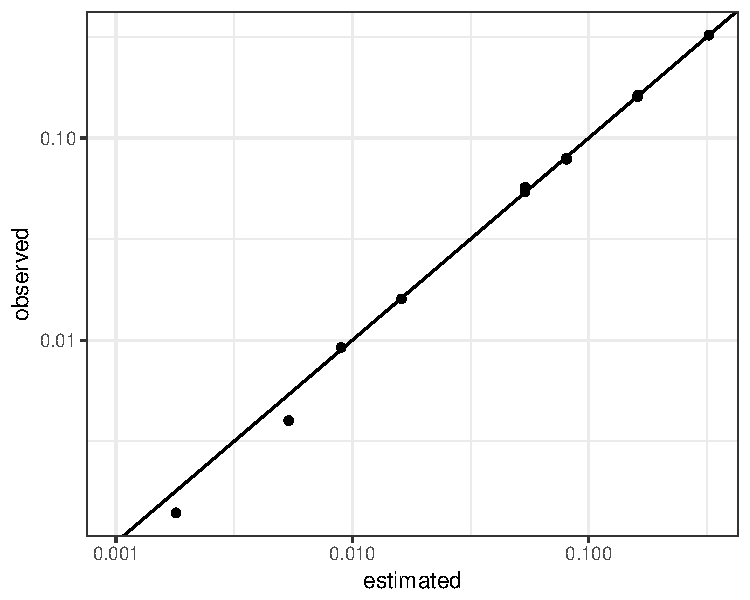
\includegraphics[width=0.8\textwidth]{figure/ex3plot-1} 

\end{knitrout}

\section{Fitting}

\subsection{Preliminaries}
\begin{knitrout}
\definecolor{shadecolor}{rgb}{0.969, 0.969, 0.969}\color{fgcolor}\begin{kframe}
\begin{alltt}
\hlkwd{source}\hlstd{(}\hlstr{"mosqfuns2.R"}\hlstd{)}
\end{alltt}
\end{kframe}
\end{knitrout}
The only part of the log-likelihood
that depends on $B$ (or $s_0$, which implicitly depends on $B$
via $s_0=B-K$) is
$$
-M \log B + \log B! - \log (B-K)!
$$
In other words, $K$ is a sufficient statistic for estimating $B$ 
by maximum likelihood.  (Alternatively, we can estimate $B$ via
the method of moments, since we can calculate an expected value for
$K$: the answers turn out to be quite similar.)

We will try four different estimates: two depend (only) on $K$,
one on the probability of doublets ($W$), one on the time to
first collision $\tau_0$.  In each case we will compute the
probability distribution of the summary statistic for
$B=40$, $M=20$, calculate the estimated value of $B$ for each
value of the summary statistic, and calculate bias, variance,
and mean-squared error for the estimate.

First simulate probability distributions of $W$, $K$, $\tau_0$.
\begin{knitrout}
\definecolor{shadecolor}{rgb}{0.969, 0.969, 0.969}\color{fgcolor}\begin{kframe}
\begin{alltt}
\hlstd{Kfun} \hlkwb{<-} \hlkwa{function}\hlstd{(}\hlkwc{B}\hlstd{,}\hlkwc{M}\hlstd{) \{}
    \hlkwd{unname}\hlstd{(B}\hlopt{-}\hlkwd{sfun}\hlstd{(B,M,}\hlkwc{collapse}\hlstd{=}\hlnum{FALSE}\hlstd{)[}\hlnum{1}\hlstd{])}
\hlstd{\}}
\end{alltt}
\end{kframe}
\end{knitrout}

Compute doublets:
\begin{knitrout}
\definecolor{shadecolor}{rgb}{0.969, 0.969, 0.969}\color{fgcolor}\begin{kframe}
\begin{alltt}
\hlstd{Wfun} \hlkwb{<-} \hlkwa{function}\hlstd{(}\hlkwc{B}\hlstd{,}\hlkwc{M}\hlstd{) \{}
    \hlstd{v} \hlkwb{<-} \hlkwd{vfun}\hlstd{(B,M)}
    \hlkwd{sum}\hlstd{(v}\hlopt{*}\hlstd{(v}\hlopt{-}\hlnum{1}\hlstd{))}
\hlstd{\}}
\end{alltt}
\end{kframe}
\end{knitrout}

Compute time of first collision:
\begin{knitrout}
\definecolor{shadecolor}{rgb}{0.969, 0.969, 0.969}\color{fgcolor}\begin{kframe}
\begin{alltt}
\hlstd{Cfun} \hlkwb{<-} \hlkwa{function}\hlstd{(}\hlkwc{B}\hlstd{,}\hlkwc{ssize}\hlstd{=}\hlnum{2}\hlopt{*}\hlstd{B) \{}
    \hlstd{ss} \hlkwb{<-} \hlkwd{sample}\hlstd{(B,}\hlkwc{size}\hlstd{=ssize,}\hlkwc{replace}\hlstd{=}\hlnum{TRUE}\hlstd{)}
    \hlkwd{min}\hlstd{(}\hlkwd{which}\hlstd{(}\hlkwd{duplicated}\hlstd{(ss)))}
\hlstd{\}}
\end{alltt}
\end{kframe}
\end{knitrout}

\fixme{use set.seed()? fix downstream stuff so this part
can be run out of order?}
\begin{knitrout}
\definecolor{shadecolor}{rgb}{0.969, 0.969, 0.969}\color{fgcolor}\begin{kframe}
\begin{alltt}
\hlstd{nsim} \hlkwb{<-} \hlnum{1000}\hlstd{; M} \hlkwb{<-} \hlnum{20}\hlstd{; B} \hlkwb{<-} \hlnum{40}
\hlstd{Kvec} \hlkwb{<-} \hlkwd{replicate}\hlstd{(nsim,}\hlkwd{Kfun}\hlstd{(B,M))}
\hlstd{Wvec} \hlkwb{<-} \hlkwd{replicate}\hlstd{(nsim,}\hlkwd{Wfun}\hlstd{(B,M))}
\hlstd{Cvec} \hlkwb{<-} \hlkwd{replicate}\hlstd{(nsim,}\hlkwd{Cfun}\hlstd{(B))}
\end{alltt}
\end{kframe}
\end{knitrout}

\begin{knitrout}
\definecolor{shadecolor}{rgb}{0.969, 0.969, 0.969}\color{fgcolor}\begin{kframe}
\begin{alltt}
\hlstd{Ktab} \hlkwb{<-} \hlkwd{table}\hlstd{(Kvec)}\hlopt{/}\hlstd{nsim}
\hlkwd{plot}\hlstd{(Ktab)}
\end{alltt}
\end{kframe}
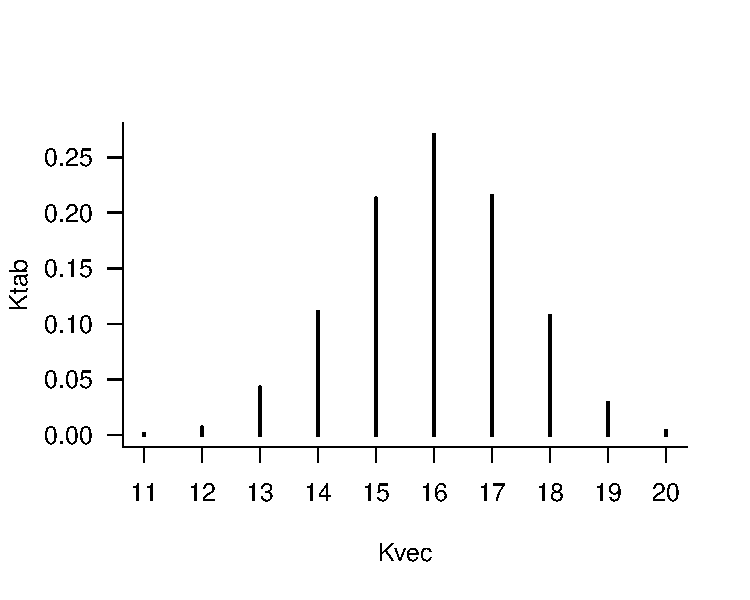
\includegraphics[width=0.8\textwidth]{figure/Ktab-1} 
\begin{kframe}\begin{alltt}
\hlstd{Kvec2} \hlkwb{<-} \hlkwd{as.numeric}\hlstd{(}\hlkwd{names}\hlstd{(Ktab))}
\end{alltt}
\end{kframe}
\end{knitrout}

\fixme{store SD and RMSE rather than var and MSE?}
\begin{knitrout}
\definecolor{shadecolor}{rgb}{0.969, 0.969, 0.969}\color{fgcolor}\begin{kframe}
\begin{alltt}
\hlstd{estres} \hlkwb{<-} \hlkwd{matrix}\hlstd{(}\hlnum{NA}\hlstd{,}\hlkwc{nrow}\hlstd{=}\hlnum{4}\hlstd{,}\hlkwc{ncol}\hlstd{=}\hlnum{3}\hlstd{,}
                 \hlkwc{dimnames}\hlstd{=}\hlkwd{list}\hlstd{(}\hlkwd{c}\hlstd{(}\hlstr{"MM"}\hlstd{,}\hlstr{"MLE"}\hlstd{,}\hlstr{"doublets"}\hlstd{,}\hlstr{"collision"}\hlstd{),}
                 \hlkwd{c}\hlstd{(}\hlstr{"bias"}\hlstd{,}\hlstr{"var"}\hlstd{,}\hlstr{"MSE"}\hlstd{)))}
\end{alltt}
\end{kframe}
\end{knitrout}

\subsection{Method of moments}

Based on binomial or Poisson approximations,
we should have the expected value of $K$ ($\hat K$) equal to
approximately $B(1-(1-(1/B))^M)$, or (in another approximation,
based on $M$, $B$ both large) $B(1-\exp(-M/B))$ (or even more
approximately) $M$: the last one recovers the case where $B \gg M$,
so we expected each mosquito to bite a different bird \ldots

The \verb+Bhat_approx+ function implements a root-finding
solution to find a method-of-moments estimate for $B$ based on known
$K$ and $M$.


\begin{knitrout}
\definecolor{shadecolor}{rgb}{0.969, 0.969, 0.969}\color{fgcolor}\begin{kframe}
\begin{alltt}
\hlstd{B_true} \hlkwb{<-} \hlnum{40}
\hlstd{Bhat_mm} \hlkwb{<-} \hlkwd{sapply}\hlstd{(Kvec2[Kvec2}\hlopt{<}\hlnum{20}\hlstd{],Bhat_approx,}\hlkwc{M}\hlstd{=}\hlnum{20}\hlstd{)}
\hlstd{B_mean_mm} \hlkwb{<-} \hlkwd{sum}\hlstd{(Bhat_mm}\hlopt{*}\hlstd{Ktab[Kvec2}\hlopt{<}\hlnum{20}\hlstd{])}
\hlstd{estres[}\hlstr{"MM"}\hlstd{,}\hlstr{"bias"}\hlstd{]} \hlkwb{<-} \hlstd{bias_mm} \hlkwb{<-} \hlstd{B_mean_mm} \hlopt{-}\hlstd{B_true}
\hlstd{estres[}\hlstr{"MM"}\hlstd{,}\hlstr{"var"}\hlstd{]} \hlkwb{<-} \hlkwd{sum}\hlstd{((Bhat_mm}\hlopt{-}\hlstd{B_mean_mm)}\hlopt{^}\hlnum{2}\hlopt{*}\hlstd{Ktab[Kvec2}\hlopt{<}\hlnum{20}\hlstd{])}
\hlstd{estres[}\hlstr{"MM"}\hlstd{,}\hlstr{"MSE"}\hlstd{]} \hlkwb{<-} \hlkwd{sum}\hlstd{((Bhat_mm}\hlopt{-}\hlstd{B_true)}\hlopt{^}\hlnum{2}\hlopt{*}\hlstd{Ktab[Kvec2}\hlopt{<}\hlnum{20}\hlstd{])}
\end{alltt}
\end{kframe}
\end{knitrout}

\subsection{MLE/likelihood ratio test}
We can compute $P(B+1)/P(B)$ (and get a relatively simple
expression that we try to equate to 1), or by brute force:

\begin{knitrout}
\definecolor{shadecolor}{rgb}{0.969, 0.969, 0.969}\color{fgcolor}\begin{kframe}


{\ttfamily\noindent\color{warningcolor}{\#\# Warning: package 'bbmle' was built under R version 3.2.5}}

{\ttfamily\noindent\color{warningcolor}{\#\# Warning: replacing previous import by 'stats::na.omit' when loading 'bbmle'}}\end{kframe}
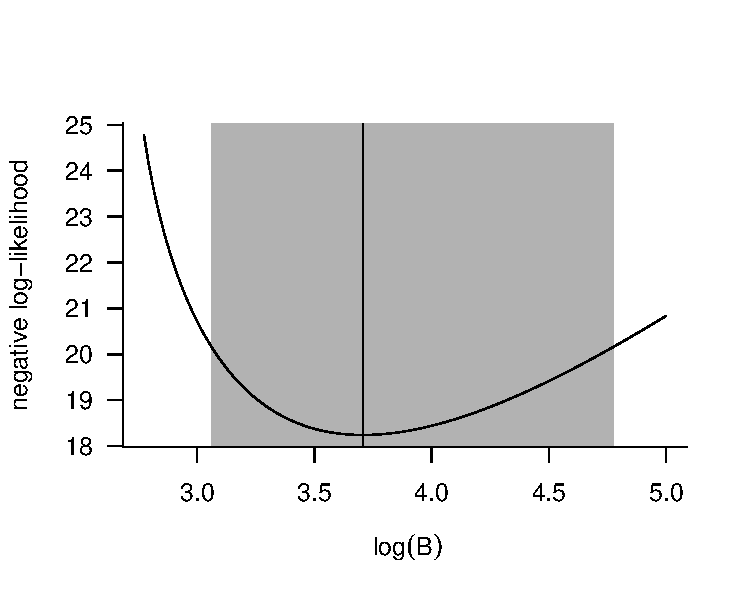
\includegraphics[width=0.8\textwidth]{figure/unnamed-chunk-1-1} 

\end{knitrout}

The gray region shows the 95\% LRT confidence intervals
($B$ such that $-\log L < -\log L_{\mbox{\small min}} + 1.92$).
Note we seem to have a computational
problem for these functions when evaluating the log-likelihood
for $\log B > 33$,
because $K/B \ll 1$. However, we really
should never be dealing with host population sizes
as large as $e^{33}$=\ensuremath{2.1464358\times 10^{14}}!


\begin{knitrout}
\definecolor{shadecolor}{rgb}{0.969, 0.969, 0.969}\color{fgcolor}\begin{kframe}
\begin{alltt}
\hlcom{## for lower bound when K=100}
\hlstd{lboundfun} \hlkwb{<-} \hlkwa{function}\hlstd{(}\hlkwc{M}\hlstd{) \{}
    \hlkwd{uniroot}\hlstd{(}\hlkwa{function}\hlstd{(}\hlkwc{x}\hlstd{)} \hlkwd{nllfun}\hlstd{(x,}\hlkwc{K}\hlstd{=M,}\hlkwc{M}\hlstd{=M)}\hlopt{-}\hlnum{1.92}\hlstd{,}
            \hlkwc{interval}\hlstd{=}\hlkwd{c}\hlstd{(}\hlkwd{log}\hlstd{(M}\hlopt{+}\hlnum{0.001}\hlstd{),}\hlnum{25}\hlstd{))}\hlopt{$}\hlstd{root}
\hlstd{\}}
\hlstd{ffun} \hlkwb{<-} \hlkwa{function}\hlstd{(}\hlkwc{K}\hlstd{,}\hlkwc{M}\hlstd{) \{}
    \hlkwa{if} \hlstd{(K}\hlopt{<}\hlstd{M) \{}
        \hlstd{f} \hlkwb{<-} \hlkwd{try}\hlstd{(}\hlkwd{fitB}\hlstd{(K,M),}\hlkwc{silent}\hlstd{=}\hlnum{TRUE}\hlstd{)}
        \hlkwa{if} \hlstd{(}\hlkwd{inherits}\hlstd{(f,}\hlstr{"try-error"}\hlstd{))} \hlkwd{rep}\hlstd{(}\hlnum{NA}\hlstd{,}\hlnum{3}\hlstd{)} \hlkwa{else} \hlkwd{unlist}\hlstd{(f)}
    \hlstd{\}} \hlkwa{else} \hlstd{\{}
        \hlkwd{c}\hlstd{(}\hlnum{NA}\hlstd{,}\hlkwd{lboundfun}\hlstd{(M),}\hlnum{NA}\hlstd{)}
    \hlstd{\}}
\hlstd{\}}
\end{alltt}
\end{kframe}
\end{knitrout}
\begin{knitrout}
\definecolor{shadecolor}{rgb}{0.969, 0.969, 0.969}\color{fgcolor}\begin{kframe}
\begin{alltt}
\hlstd{rfit} \hlkwb{<-} \hlkwd{laply}\hlstd{(Kvec2,ffun,}\hlkwc{M}\hlstd{=}\hlnum{20}\hlstd{)}
\end{alltt}
\end{kframe}
\end{knitrout}
(We get \code{NA} if $K=M$ --- of course, since
in this case $\hat B \to \infty$ --- although we should
still be able to get a lower bound in this case and hence
include it in the coverage statistics, although if we include
it in the bias calculation we will be in trouble.  In the
appropriate asymptotic case will the probability of this
case go to zero fast enough??)

\subsection{Doublets}

This is based on \cite{good_studies_1979} (\S10, ``The repeat rate''):
more generally these estimators are (apparently) known
as ``Good-Turing estimators'', e.g. \cite{mcallester_convergence_2000}:
\begin{quote}
  The total probability mass of the words not in the sample is the
  so-called missing mass. Good showed that the fraction of the sample
  consisting of words that occur only once in the sample is a nearly
  unbiased estimate of the missing mass. Here, we give a PAC-style
  high-probability confidence interval for the actual missing
  mass. More generally, for $k>0$, we give a confidence interval for the
  true probability mass of the set of words occuring $k$ times in the
  sample.
\end{quote}

There is also other relevant literature in ecology, mostly from
the point of view of species distribution estimation
\citep{good_population_1953,chao_estimating_1992} --- maybe
a good place to go to get procedures for estimating confidence
intervals \ldots

Letting $p_1,...p_B$ be the probabilities of each bird occuring within the sample, if $p_1=...=p_B = 1/B$ (the equally likely or equiprobability assumption), the repeat rate reduces to a expression only involving the parameter, $B$.

The sum of doublets, $W=\sum v_i (v_i-1)$, (where $V = \{v_i\} = $ the unordered occupancy of birds) has an
expected value

$W = \frac{\{M(M-1)\}}{\hat{B}}$
hence $\hat{B} = W / \{M(M-1)\}$

\begin{knitrout}
\definecolor{shadecolor}{rgb}{0.969, 0.969, 0.969}\color{fgcolor}\begin{kframe}
\begin{alltt}
\hlstd{Wtab} \hlkwb{<-} \hlkwd{table}\hlstd{(Wvec)}\hlopt{/}\hlstd{nsim}
\hlstd{Wvec2} \hlkwb{<-} \hlkwd{as.numeric}\hlstd{(}\hlkwd{names}\hlstd{(Wtab))}
\hlstd{Bhat_doublet}\hlkwb{<-}\hlstd{M}\hlopt{*}\hlstd{(M}\hlopt{-}\hlnum{1}\hlstd{)}\hlopt{/}\hlstd{Wvec2}
\hlkwd{plot}\hlstd{(Wvec2,Bhat_doublet,}\hlkwc{xlab}\hlstd{=}\hlstr{"doublet statistic"}\hlstd{,}\hlkwc{ylab}\hlstd{=}\hlstr{"estimated B"}\hlstd{)}
\end{alltt}
\end{kframe}
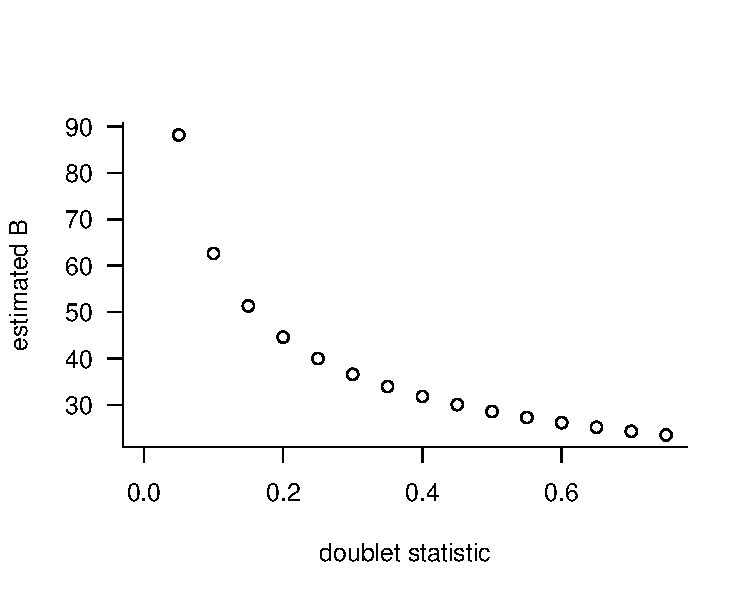
\includegraphics[width=0.8\textwidth]{figure/unnamed-chunk-2-1} 

\end{knitrout}

\subsection{time to first collision}
\begin{knitrout}
\definecolor{shadecolor}{rgb}{0.969, 0.969, 0.969}\color{fgcolor}\begin{kframe}
\begin{alltt}
\hlstd{Texpfun} \hlkwb{<-} \hlkwa{function}\hlstd{(}\hlkwc{B}\hlstd{,}\hlkwc{maxn}\hlstd{=}\hlnum{4}\hlopt{*}\hlstd{B) \{}
    \hlstd{nvec} \hlkwb{<-} \hlnum{2}\hlopt{:}\hlstd{maxn}
    \hlkwd{sum}\hlstd{(}\hlkwd{exp}\hlstd{(}\hlopt{-}\hlstd{(nvec}\hlopt{*}\hlstd{(nvec}\hlopt{-}\hlnum{1}\hlstd{))}\hlopt{/}\hlstd{(}\hlnum{2}\hlopt{*}\hlstd{B)))}
\hlstd{\}}
\hlstd{Bhat_T} \hlkwb{<-} \hlkwa{function}\hlstd{(}\hlkwc{tau}\hlstd{) \{}
    \hlkwd{uniroot}\hlstd{(}\hlkwa{function}\hlstd{(}\hlkwc{x}\hlstd{) \{ tt} \hlkwb{<-} \hlkwd{Texpfun}\hlstd{(x)}
                          \hlcom{## cat(tau,tt,"\textbackslash{}n")}
                          \hlstd{tt}\hlopt{-}\hlstd{tau \},}
            \hlkwc{interval}\hlstd{=}\hlkwd{c}\hlstd{(tau,}\hlnum{1e6}\hlstd{))}\hlopt{$}\hlstd{root}
\hlstd{\}}
\hlstd{Ctab} \hlkwb{<-} \hlkwd{table}\hlstd{(Cvec)}\hlopt{/}\hlstd{nsim}
\hlstd{Cvec2} \hlkwb{<-} \hlkwd{as.numeric}\hlstd{(}\hlkwd{names}\hlstd{(Ctab))}
\end{alltt}
\end{kframe}
\end{knitrout}

\begin{knitrout}
\definecolor{shadecolor}{rgb}{0.969, 0.969, 0.969}\color{fgcolor}\begin{kframe}
\begin{alltt}
\hlstd{Bhat_collision} \hlkwb{<-} \hlkwd{sapply}\hlstd{(Cvec2,Bhat_T)}
\end{alltt}
\end{kframe}
\end{knitrout}

\subsection{Results}
Plot results for each value of $K$, with spacing on the
horizontal axis corresponding to the probability distribution
of $K$ (the lower part of the confidence interval for $K=100$
is drawn in light blue):

\begin{knitrout}
\definecolor{shadecolor}{rgb}{0.969, 0.969, 0.969}\color{fgcolor}
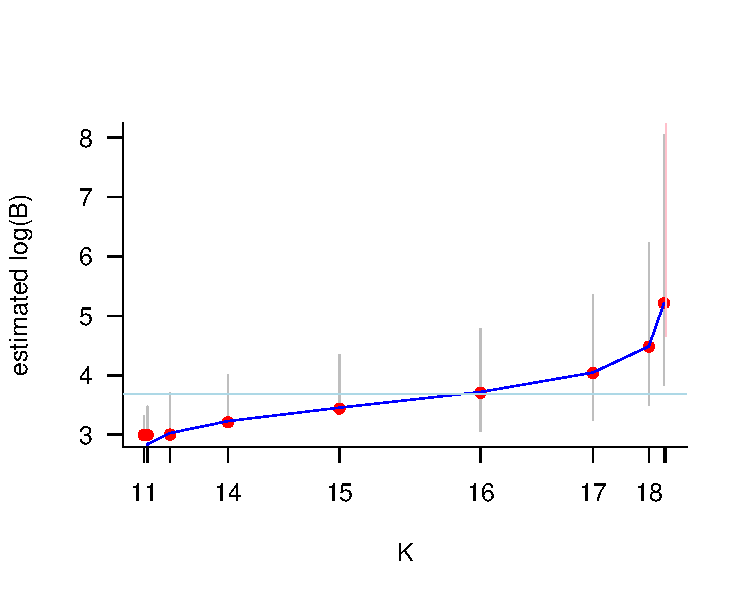
\includegraphics[width=0.8\textwidth]{figure/coverplot-1} 

\end{knitrout}

Coverage (nominal value is 0.95):
\begin{knitrout}
\definecolor{shadecolor}{rgb}{0.969, 0.969, 0.969}\color{fgcolor}\begin{kframe}
\begin{alltt}
\hlkwd{sum}\hlstd{(Ktab}\hlopt{*}\hlstd{(rfit[,}\hlnum{2}\hlstd{]}\hlopt{<}\hlkwd{log}\hlstd{(B)} \hlopt{&} \hlstd{rfit[,}\hlnum{3}\hlstd{]}\hlopt{>}\hlkwd{log}\hlstd{(B)),}\hlkwc{na.rm}\hlstd{=}\hlnum{TRUE}\hlstd{)}
\end{alltt}
\begin{verbatim}
## [1] 0.592
\end{verbatim}
\end{kframe}
\end{knitrout}
Not bad (somewhat conservative).

Compare with fitting $P(B+1)/P(B) = ( 1+ 1/B )^M (1-K/(B+1))=1$
(probably faster: not really susceptible to closed-form solution either).

\begin{knitrout}
\definecolor{shadecolor}{rgb}{0.969, 0.969, 0.969}\color{fgcolor}\begin{kframe}
\begin{alltt}
\hlstd{rKfun} \hlkwb{<-} \hlkwa{function}\hlstd{(}\hlkwc{B}\hlstd{,}\hlkwc{K}\hlstd{,}\hlkwc{M}\hlstd{) \{}
    \hlstd{(}\hlnum{1}\hlopt{+}\hlnum{1}\hlopt{/}\hlstd{B)}\hlopt{^}\hlstd{M}\hlopt{*}\hlstd{(}\hlnum{1}\hlopt{-}\hlstd{K}\hlopt{/}\hlstd{(B}\hlopt{+}\hlnum{1}\hlstd{))}\hlopt{-}\hlnum{1}
\hlstd{\}}
\hlstd{u1} \hlkwb{<-} \hlkwd{uniroot}\hlstd{(rKfun,}\hlkwc{interval}\hlstd{=}\hlkwd{c}\hlstd{(}\hlnum{16}\hlstd{,}\hlnum{1e6}\hlstd{),}\hlkwc{K}\hlstd{=}\hlnum{16}\hlstd{,}\hlkwc{M}\hlstd{=}\hlnum{20}\hlstd{)}
\hlkwd{log}\hlstd{(u1}\hlopt{$}\hlstd{root)}
\end{alltt}
\begin{verbatim}
## [1] 3.695131
\end{verbatim}
\begin{alltt}
\hlkwd{fitB}\hlstd{(}\hlnum{16}\hlstd{,}\hlnum{20}\hlstd{)}
\end{alltt}
\begin{verbatim}
## $fit
##     logB 
## 3.707357 
## 
## $confint
##    2.5 %   97.5 % 
## 3.061193 4.775601
\end{verbatim}
\end{kframe}
\end{knitrout}
Actually not quite identical --- precision problems?

Approximations:
\begin{equation*}
  \begin{split}
    \left( 1+ 1/B\right)^M (1-K/(B+1)) & \approx e^{M/B} (1-K/(B+1))
  \qquad (B, M \gg 1) \\
  & \approx e^{M/B} (1-K/B) \qquad (B \gg 1)
\end{split}
\end{equation*}

Probably a fine approximation, but not sure that we can 
get much more out of this without a much more extreme
approximation like $e^{M/B} \approx 1+(M/B)$ --- would
be nice if we could use Lambert $W$ but I don't see how.

\subsection{Simulation results}


\begin{knitrout}
\definecolor{shadecolor}{rgb}{0.969, 0.969, 0.969}\color{fgcolor}
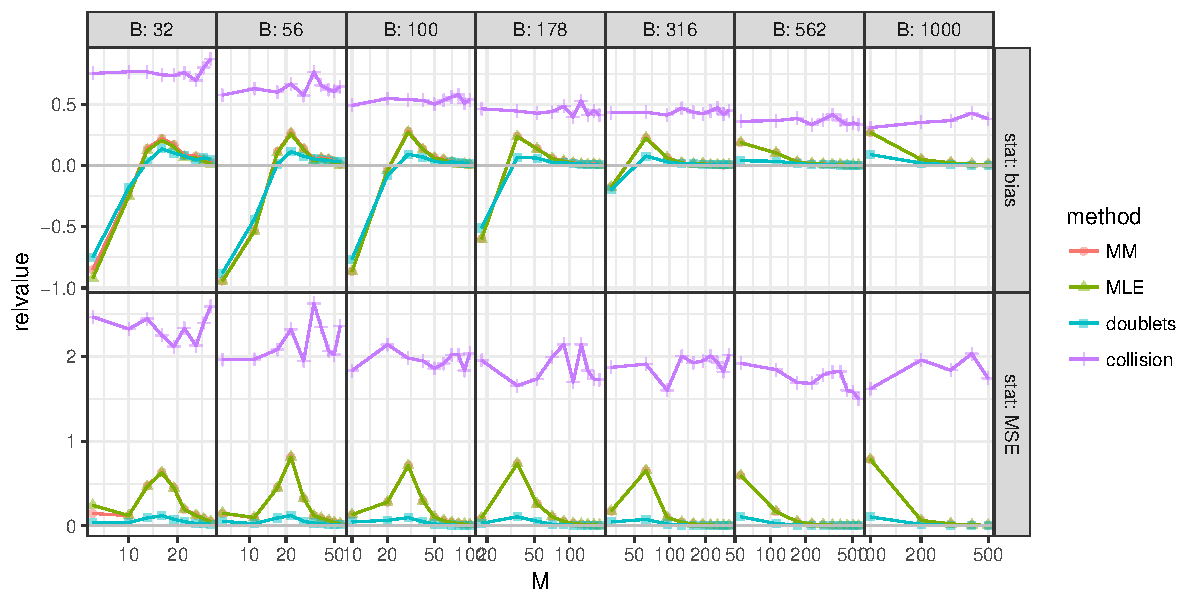
\includegraphics[width=\textwidth]{figure/simplot1-1} 

\end{knitrout}

Take out first-collision method and $M>10$:

\begin{knitrout}
\definecolor{shadecolor}{rgb}{0.969, 0.969, 0.969}\color{fgcolor}
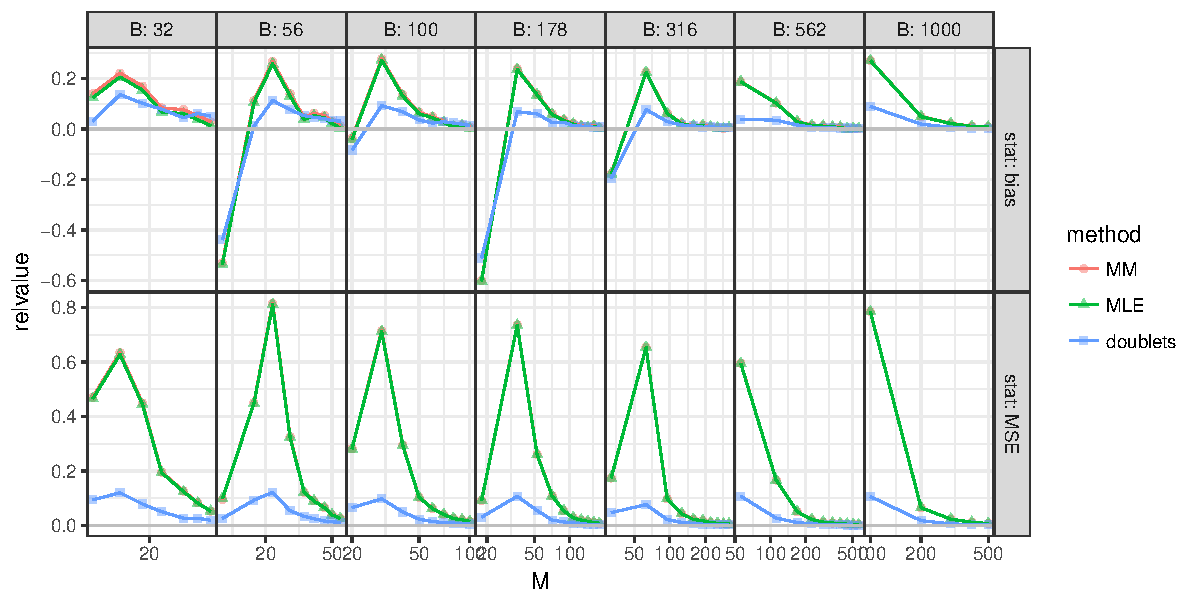
\includegraphics[width=\textwidth]{figure/simplot2-1} 

\end{knitrout}

Zoom in further (doublets only, value $>0$, $M>20$):

\begin{knitrout}
\definecolor{shadecolor}{rgb}{0.969, 0.969, 0.969}\color{fgcolor}
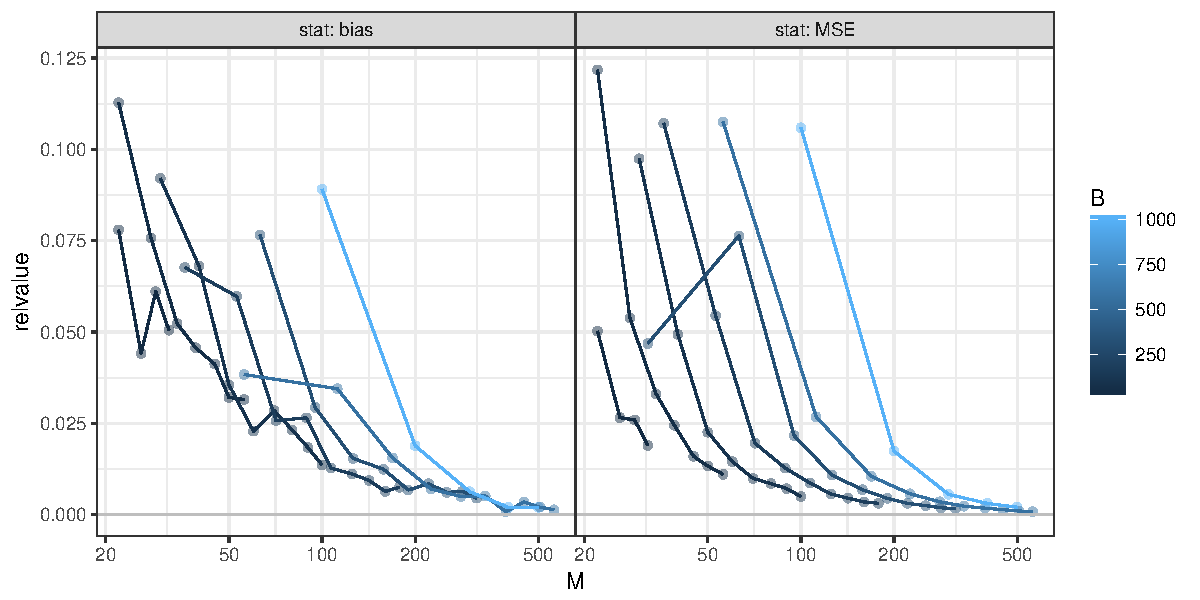
\includegraphics[width=\textwidth]{figure/simplot3-1} 

\end{knitrout}

The time-to-first-collision method is terrible (although I can't rule
out the possibility that I made a mistake).  Somewhat to my surprise,
the doublet method seems to dominate.  There is some severe negative
bias for particular combinations of low $M$ and intermediate $B$,
although I should again double-check and make sure that something
funny isn't going on (also note that the $K=M$ results might be
excluded from some of the calculations).  I could look in more detail
at the distributions of $K$ and $W$ for those cases, to see what's
going on \ldots 
\begin{itemize}
  \item Bias reduction methods??  
  \item Rules of thumb for keeping MSE below some threshold (in terms
    of $M$ or $M/B$)?
  \item Why do bias and MSE for MLE/MM have an intermediate peak?
  \item Should work out confidence intervals for the doublet method
\end{itemize}



\section{Probability of collision}
As before, we know that $P(K=M)$ is $\prod_{i=0}^{M-1} (B-i)/B$.
This is useful in and of itself.  If we have a preliminary
estimate of the bird population size, 
how big do we have to make the sample
size $M$ to get a specified probability of collision?
\begin{knitrout}
\definecolor{shadecolor}{rgb}{0.969, 0.969, 0.969}\color{fgcolor}\begin{kframe}
\begin{alltt}
\hlstd{collision_prob} \hlkwb{<-} \hlkwa{function}\hlstd{(}\hlkwc{M}\hlstd{,}\hlkwc{B}\hlstd{,}\hlkwc{inverse}\hlstd{=}\hlnum{FALSE}\hlstd{,}\hlkwc{log}\hlstd{=}\hlnum{FALSE}\hlstd{) \{}
    \hlstd{r} \hlkwb{<-} \hlkwd{sum}\hlstd{(}\hlkwd{log}\hlstd{(B}\hlopt{-}\hlkwd{seq}\hlstd{(}\hlnum{0}\hlstd{,M}\hlopt{-}\hlnum{1}\hlstd{)))}\hlopt{-}\hlstd{M}\hlopt{*}\hlkwd{log}\hlstd{(B)}
    \hlkwa{if} \hlstd{(inverse) \{}
        \hlkwa{if} \hlstd{(log) r} \hlkwa{else} \hlkwd{exp}\hlstd{(r)}
    \hlstd{\}} \hlkwa{else} \hlstd{\{}
        \hlstd{r2} \hlkwb{<-} \hlnum{1}\hlopt{-}\hlkwd{exp}\hlstd{(r)}
        \hlkwa{if} \hlstd{(log)} \hlkwd{log}\hlstd{(r2)} \hlkwa{else} \hlstd{r2}
    \hlstd{\}}
\hlstd{\}}
\end{alltt}
\end{kframe}
\end{knitrout}
Approximation for $M \ll B$ ?

\begin{knitrout}
\definecolor{shadecolor}{rgb}{0.969, 0.969, 0.969}\color{fgcolor}
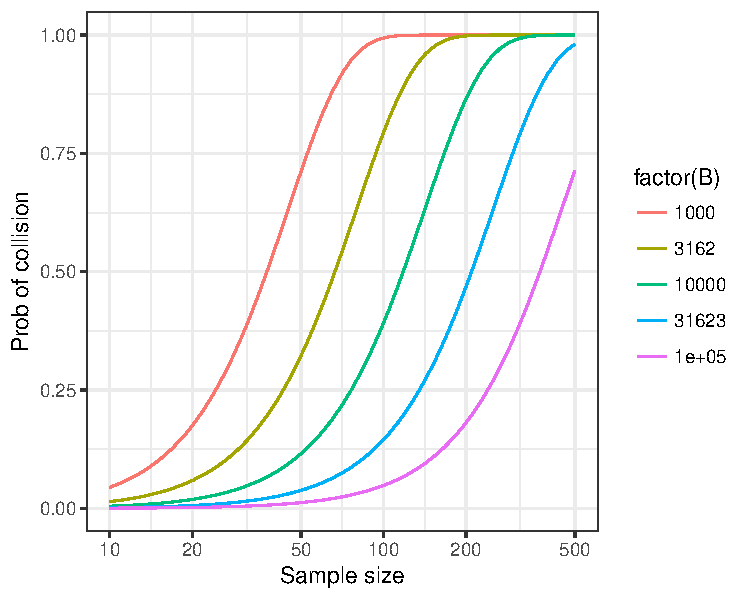
\includegraphics[width=0.8\textwidth]{figure/collision_approx-1} 

\end{knitrout}


\section{Lower bound on $B$ when $K=M$}

This is a little dodgy, but: when $K=M$, the MLE $\hat B$
goes to infinity, because $-M \log B + \log B! - \log (B-K)!$
is maximized as $B \to \infty$.

\begin{knitrout}
\definecolor{shadecolor}{rgb}{0.969, 0.969, 0.969}\color{fgcolor}
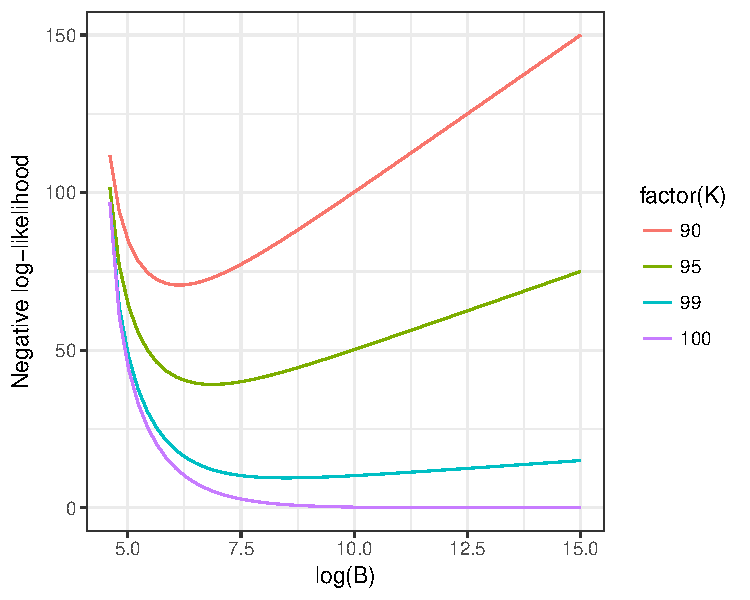
\includegraphics[width=0.8\textwidth]{figure/lplot1-1} 

\end{knitrout}

However, we can still try to solve for the case where 
$-\log L=\chi^2_1(0.975)/2=1.92$ to get a lower bound.
For example, if $M=K=100$,
\begin{knitrout}
\definecolor{shadecolor}{rgb}{0.969, 0.969, 0.969}\color{fgcolor}\begin{kframe}
\begin{alltt}
\hlstd{lobound} \hlkwb{<-} \hlkwd{uniroot}\hlstd{(}\hlkwa{function}\hlstd{(}\hlkwc{x}\hlstd{)} \hlkwd{nllfun}\hlstd{(x,}\hlkwc{K}\hlstd{=}\hlnum{100}\hlstd{,}\hlkwc{M}\hlstd{=}\hlnum{100}\hlstd{)}\hlopt{-}\hlnum{1.92}\hlstd{,}
   \hlkwc{interval}\hlstd{=}\hlkwd{c}\hlstd{(}\hlkwd{log}\hlstd{(}\hlnum{101}\hlstd{),}\hlnum{25}\hlstd{))}\hlopt{$}\hlstd{root}
\end{alltt}
\end{kframe}
\end{knitrout}
So in this case (for $M=100$, $K=100$) 
our 95\% lower bound on the population size
is $B=2611$ (this leaves
open the question of whether profile confidence
limits are reasonable in this case).

Here's a more general result:
\begin{knitrout}
\definecolor{shadecolor}{rgb}{0.969, 0.969, 0.969}\color{fgcolor}\begin{kframe}
\begin{alltt}
\hlstd{lboundfun} \hlkwb{<-} \hlkwa{function}\hlstd{(}\hlkwc{M}\hlstd{) \{}
    \hlkwd{uniroot}\hlstd{(}\hlkwa{function}\hlstd{(}\hlkwc{x}\hlstd{)} \hlkwd{nllfun}\hlstd{(x,}\hlkwc{K}\hlstd{=M,}\hlkwc{M}\hlstd{=M)}\hlopt{-}\hlnum{1.92}\hlstd{,}
            \hlkwc{interval}\hlstd{=}\hlkwd{c}\hlstd{(}\hlkwd{log}\hlstd{(M}\hlopt{+}\hlnum{0.001}\hlstd{),}\hlnum{25}\hlstd{))}\hlopt{$}\hlstd{root}
\hlstd{\}}
\hlstd{Mvec} \hlkwb{<-} \hlkwd{round}\hlstd{(}\hlnum{10}\hlopt{^}\hlkwd{seq}\hlstd{(}\hlnum{1}\hlstd{,}\hlnum{4}\hlstd{,}\hlkwc{length}\hlstd{=}\hlnum{31}\hlstd{))}
\hlstd{dd3} \hlkwb{<-} \hlkwd{data.frame}\hlstd{(}\hlkwc{M}\hlstd{=Mvec,}\hlkwc{lo}\hlstd{=}\hlkwd{exp}\hlstd{(}\hlkwd{sapply}\hlstd{(Mvec,lboundfun)))}
\hlkwd{ggplot}\hlstd{(dd3,}\hlkwd{aes}\hlstd{(M,lo))}\hlopt{+}\hlkwd{geom_line}\hlstd{()}\hlopt{+}
    \hlkwd{scale_y_log10}\hlstd{(}\hlkwc{breaks}\hlstd{=}\hlnum{10}\hlopt{^}\hlstd{(}\hlnum{2}\hlopt{:}\hlnum{7}\hlstd{))}\hlopt{+}
    \hlkwd{scale_x_log10}\hlstd{(}\hlkwc{breaks}\hlstd{=}\hlnum{10}\hlopt{^}\hlstd{(}\hlnum{1}\hlopt{:}\hlnum{4}\hlstd{))}\hlopt{+}
    \hlkwd{labs}\hlstd{(}\hlkwc{x}\hlstd{=}\hlstr{"sample size"}\hlstd{,}\hlkwc{y}\hlstd{=}\hlstr{"lower bound on population size"}\hlstd{)}
\end{alltt}
\end{kframe}
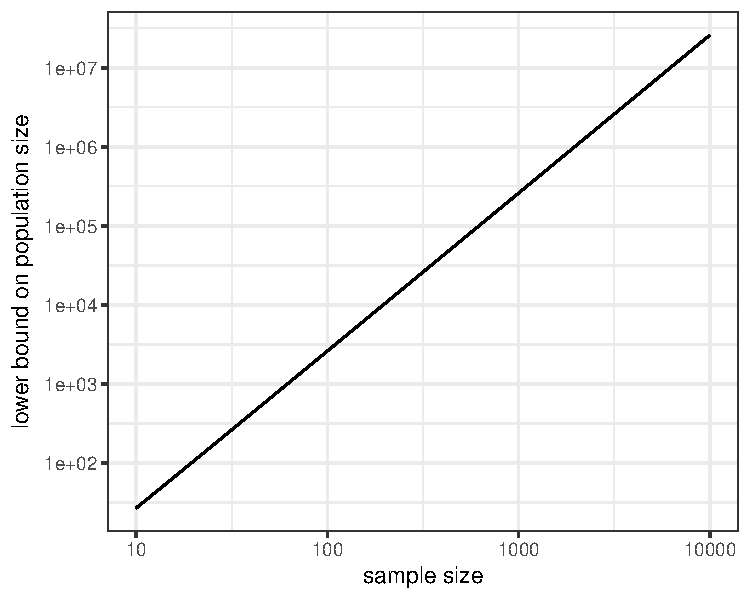
\includegraphics[width=0.8\textwidth]{figure/lbound-1} 

\end{knitrout}
This is a perfectly boring graph, with log-log slope nearly
exactly 2.0  --- a quadratic relationship between the lower bound and the size
of $M$ (this should be easy to work out analytically, or to argue
heuristically?)

\section{To do}

\begin{itemize}
  \item Theoretical justification for using MLE, and
    profile likelihood CI: in what limit are we working --- what
    gets large (i.e. $B$, $M$, $K$, $s_0$)?  In general we can
    expect $B \approx s_0 \gg M \approx K$ \ldots  Can we show
    that something converges appropriately to give us 
    asymptotic consistency, $\chi^2$ distribution of deviance,
    etc.?  
  \item Get the theoretical distribution
    of $K$ (hypergeometric??), which might allow us to compute bias
    for particular cases by brute force, and make a case about
    asymptotic stuff?  (If we know the distribution of $K$ then
    we also know the distribution of $\hat B$, by inversion \ldots)
  \item Could probably get confidence limits considerably quicker
    by root-finding rather than using the general \code{mle2}
    machinery?
  \item Might be able to do more exact/more justifiable confidence
    limits on $B$ by evaluating the spectrum of probabilities of
    no-collision as a function of $B$?
\end{itemize}

\section{Data (!!)}

OK, now we actually have a little bit of information about
plausible sizes of $B$, $M$ \ldots

The actual $B$ values (number of American robins at a site)
are thought to be in the range 10--40
(much smaller than I was imagining).

Some values of $M$ from three sites across a range of years:
\begin{knitrout}
\definecolor{shadecolor}{rgb}{0.969, 0.969, 0.969}\color{fgcolor}\begin{kframe}
\begin{verbatim}
##           site year  M
## 1 Foggy Bottom 2004 19
## 2 Foggy Bottom 2006 11
## 3 Foggy Bottom 2008 13
## 4 Foggy Bottom 2011 17
## 5    Baltimore 2008 40
## 6    Baltimore 2010 18
## 7         NMNH 2004 14
\end{verbatim}
\end{kframe}
\end{knitrout}

So if the local bird populations are really as small 
as they are thought to be, we should be very surprised
if there are no collisions: here are the collision probabilities
(i.e. the probability that at least one bird is sampled by
more than one mosquito) for $B=40$:
\begin{knitrout}
\definecolor{shadecolor}{rgb}{0.969, 0.969, 0.969}\color{fgcolor}\begin{kframe}
\begin{alltt}
\hlkwd{round}\hlstd{(}\hlkwd{sapply}\hlstd{(mdat}\hlopt{$}\hlstd{M,collision_prob,}\hlkwc{B}\hlstd{=}\hlnum{40}\hlstd{),}\hlnum{3}\hlstd{)}
\end{alltt}
\begin{verbatim}
## [1] 0.994 0.780 0.888 0.982 1.000 0.989 0.925
\end{verbatim}
\end{kframe}
\end{knitrout}
(The probability of a collision with $B=M=40$ is not
exactly 1, but it's very close: the probability of
\emph{not} having a collision is \ensuremath{6.749093\times 10^{-17}}.)

It's not clear how much power we have to distinguish different
effective population sizes from these data (i.e. we could tell
if they were much larger, but not necessarily if they're much
smaller).  For example, here are the expected $K$ distributions
from an effective population size of $B=40$ (black) and $B=20$
(red):

\begin{knitrout}
\definecolor{shadecolor}{rgb}{0.969, 0.969, 0.969}\color{fgcolor}
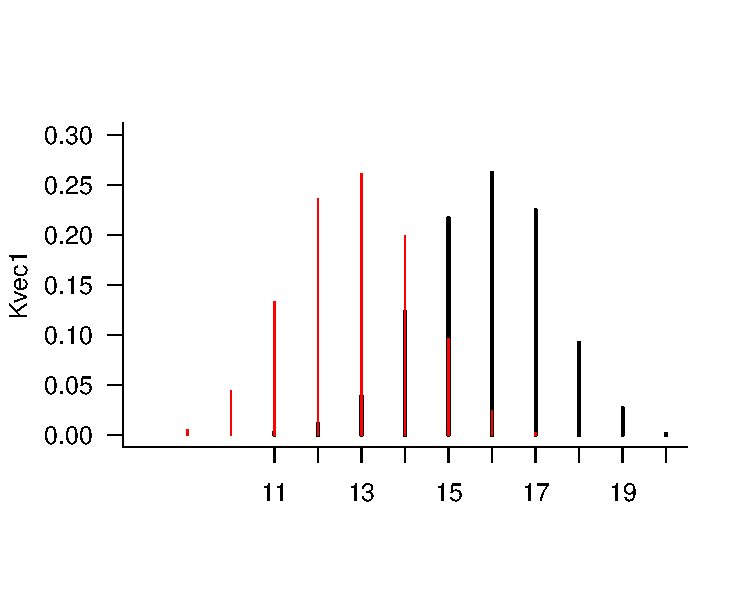
\includegraphics[width=0.8\textwidth]{figure/expkb-1} 

\end{knitrout}

For example, if we were trying to distinguish the two
hypotheses that $B=20$ vs. $B=40$:

\begin{knitrout}
\definecolor{shadecolor}{rgb}{0.969, 0.969, 0.969}\color{fgcolor}
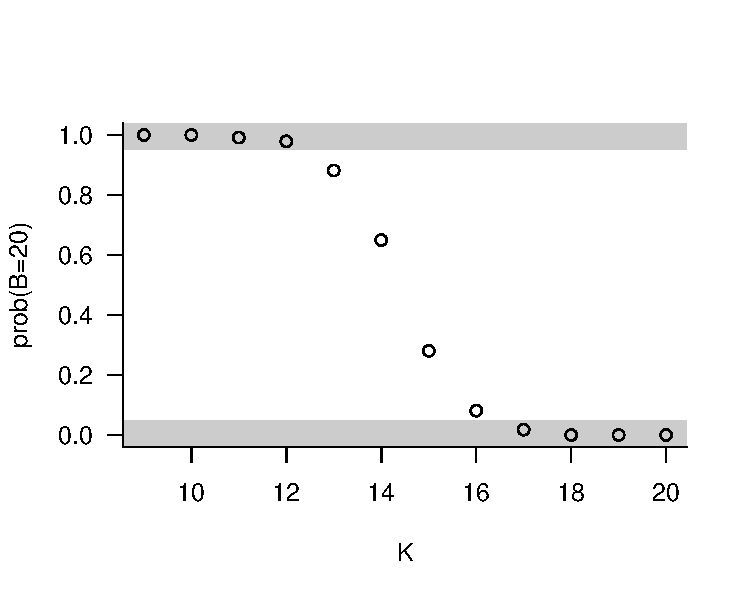
\includegraphics[width=0.8\textwidth]{figure/expkb2-1} 

\end{knitrout}
If $B$ were really 20, we would only have
a power of 0.418 to detect the difference.

\section{To do}
\begin{itemize}
\item incorporate stuff from mbrs talk
\item estimates
\item confidence intervals for doublets?
\item hierarchical models?  combinations?
\item stuff from Steve Walker, JD
\end{itemize}

\section{Junk}

\subsection{Derivatives of log-likelihood}
If we wanted to, we would in principle be able to 
use $dL/d(\log B)=-M + \psi(B) B - \psi(B-K) B$
where $\psi$ is the digamma function (although this
probably isn't worth it because we can likely solve
all our problems faster by root-finding rather than
minimization).

\begin{knitrout}
\definecolor{shadecolor}{rgb}{0.969, 0.969, 0.969}\color{fgcolor}\begin{kframe}
\begin{alltt}
\hlstd{nllgrad} \hlkwb{<-} \hlkwa{function}\hlstd{(}\hlkwc{logB}\hlstd{,}\hlkwc{K}\hlstd{,}\hlkwc{M}\hlstd{) \{}
    \hlstd{B} \hlkwb{<-} \hlkwd{exp}\hlstd{(logB)}
    \hlstd{M} \hlopt{-} \hlkwd{digamma}\hlstd{(B)}\hlopt{*}\hlstd{B}\hlopt{+}\hlkwd{digamma}\hlstd{(B}\hlopt{-}\hlstd{K)}\hlopt{*}\hlstd{B}
\hlstd{\}}
\hlkwd{grad}\hlstd{(}\hlkwa{function}\hlstd{(}\hlkwc{x}\hlstd{)} \hlkwd{nllfun}\hlstd{(x,}\hlkwc{K}\hlstd{=}\hlnum{98}\hlstd{,}\hlkwc{M}\hlstd{=}\hlnum{100}\hlstd{),}\hlkwc{x}\hlstd{=}\hlnum{7}\hlstd{)}
\end{alltt}
\begin{verbatim}
## [1] -2.609517
\end{verbatim}
\begin{alltt}
\hlkwd{nllgrad}\hlstd{(}\hlnum{7}\hlstd{,}\hlnum{98}\hlstd{,}\hlnum{100}\hlstd{)}
\end{alltt}
\begin{verbatim}
## [1] -2.707652
\end{verbatim}
\begin{alltt}
\hlkwd{grad}\hlstd{(}\hlkwa{function}\hlstd{(}\hlkwc{x}\hlstd{)} \hlkwd{nllfun}\hlstd{(x,}\hlkwc{K}\hlstd{=}\hlnum{7}\hlstd{,}\hlkwc{M}\hlstd{=}\hlnum{4}\hlstd{),}\hlkwc{x}\hlstd{=}\hlnum{3}\hlstd{)}
\end{alltt}
\begin{verbatim}
## [1] -4.344651
\end{verbatim}
\begin{alltt}
\hlkwd{nllgrad}\hlstd{(}\hlnum{3}\hlstd{,}\hlnum{7}\hlstd{,}\hlnum{4}\hlstd{)}
\end{alltt}
\begin{verbatim}
## [1] -4.879593
\end{verbatim}
\end{kframe}
\end{knitrout}
(Not quite right yet.)

\subsection{Closed-form solution for $\mbox{Prob}(K)$}

LB thinks this is difficult.

Gessel solution for $K$ (Bose-Einstein??):
$\left( \binom{B}{B-K} \binom{M-1}{K-1} \right) / \binom{B+M-1}{M}$
\begin{knitrout}
\definecolor{shadecolor}{rgb}{0.969, 0.969, 0.969}\color{fgcolor}\begin{kframe}
\begin{alltt}
\hlcom{## dhyper(B-K,B,M-1,M)}
\hlstd{myhyper} \hlkwb{<-} \hlkwa{function}\hlstd{(}\hlkwc{K}\hlstd{,}\hlkwc{M}\hlstd{,}\hlkwc{B}\hlstd{,}\hlkwc{log}\hlstd{=}\hlnum{FALSE}\hlstd{) \{}
    \hlstd{r} \hlkwb{<-} \hlkwd{lchoose}\hlstd{(B,B}\hlopt{-}\hlstd{K)}\hlopt{+}\hlkwd{lchoose}\hlstd{(M}\hlopt{-}\hlnum{1}\hlstd{,K}\hlopt{-}\hlnum{1}\hlstd{)}\hlopt{-}\hlkwd{lchoose}\hlstd{(B}\hlopt{+}\hlstd{M}\hlopt{-}\hlnum{1}\hlstd{,M)}
    \hlkwa{if} \hlstd{(log) r} \hlkwa{else} \hlkwd{exp}\hlstd{(r)}
\hlstd{\}}
\hlcom{## R notation:}
\hlcom{## H(x,m,n,k) -> choose(m,x) choose(n,k-x) / choose(m+n,k)}
\hlcom{## K=B-s_0}
\hlcom{## x=s0=B-K; m=B; n=M-1; k=M; m+n=B+M-1; k-x =M-s0}
\end{alltt}
\end{kframe}
\end{knitrout}

\section{More on Good-Turing}

Wikipedia, etc.

\bibliography{mosq}
\end{document}
